\chapter{python Porosity Uptake Correlator (pyPUC)}
\label{ch:pyPUC}

\newpage
\section*{Abstract}
For the optimal exploitation of porous materials in environmentally relevant \gls{physisorption} applications, the relationship between widths of pores within the \gls{adsorbent} and uptake capacity for the \gls{adsorbate} in question must be well understood. As these applications typically utilise the pressure-dependency of \gls{adsorption}, an understanding of the optimal pore size for uptake of the \gls{adsorbate} as a function of pressure is required. Current methods for investigating this relationship are currently limited by (i) reliance on computational modelling to approximate the result, (ii) only investigating this problem at a few discrete pressures, and often (iii) using the unsuitable measure of the `average' pore width. This work seeks to address all three of these inadequacies with the python Porosity Uptake Correlator; a software that uses experimental DataSets composed of gravimetric uptake isotherms and \acrfullpl{psd} of a group of samples that are compositionally similar, yet with diversity in terms of their porosity. Porosity (of all samples) within some pore size range is correlated to uptake of the \gls{adsorbate} at a given pressure \textit{via} linear regression. This process is then repeated for all defined pore size ranges and pressures, yielding a relationship between porosity within pores within some width range and association with improved uptake of the \gls{adsorbent} (defined by the Pearson coefficient, $r^2$).

In \ref{pub:pyPUC}, pyPUC was applied to the uptake of \ce{CO2} on \glspl{turbostratic carbon}, which gave some novel insights into this \gls{adsorption} process. Firstly, while \glspl{ultramicropore} are very important for low pressure \ce{CO2} uptake, at pressures above \qty{1.0}{\bar}, their influence diminishes significantly. However there is an indication that the traditional division of \glspl{micropore} into \glspl{ultramicropore} and \glspl{supermicropore} at \qty{7.0}{\angstrom} may not truly have physical significance to \ce{CO2} uptake. Finally, the comparative investigation of the utility of \ce{N2}, \ce{O2}, and \ce{H2} as well as the pairs \ce{N2}/\ce{H2}, and \ce{O2}/\ce{H2} as porosimetric probes for the exploration of the porosity- and pressure-dependent \ce{CO2} uptake relationship shows that traditional \ce{N2} porosimetry can be improved on as a predictor for low-pressure \ce{CO2} uptake in these materials. pyPUC shows promise in providing similarly nuanced conclusions in future applications with other \gls{adsorbate}-\gls{adsorbent} pairs.

\newpage
\section{Introduction}
While surface chemistry may play a role in small molecule \gls{adsorption},\citep{Lueking2004, Li2011a, Li2020Sustainable, wang2012significantly, Botome2017Preparation, liang2013, Kayal2018Activated} in the case of \glspl{turbostratic carbon}, porosity is the defining variable for gas uptake performance\citep{Sevilla2014Energy, Adeniran2016Is, Sevilla2013Assessment, Choi2019Unique, Lee2013Determination, Presser2011Effect, Wickramaratne2013Importance} - see \ref{pub:review}, \textbf{section 3}. While increases in overall surface area and pore volume do improve gas uptake,\citep{Cox2017Ultra, Blankenship2017Cigarette} the effects of these parameters are limited by pore size\citep{Sevilla2014Energy, Sevilla2013Assessment} \citep{Choi2019Unique, Li2019Selective, Cabria2007optimum, Gogotsi2009, Masika2012} - that is, it is important to maximise the porosity of pores with some width in order to optimise gas uptake. This so-called optimum pore width is dependent not only on the targeted sorptive,\citep{Presser2011Effect, Biloe2002Optimal, Cabria2007optimum} but on the surface chemistry\citep{wang2012significantly, Kayal2018Activated, Lueking2004} and pore geometry\citep{Rzepka1998Physisorption, Zhou2004comparative, Hlushak2018Heat} of the \gls{adsorbent}. With all of these factors controlled for, at a given temperature, optimum pore size also appears to be highly variable with pressure.\citep{Presser2011Effect, DelaCasaLillo2002Hydrogen} Up to now, the optimum pore width is defined either as (i) a single pore width\citep{Sevilla2014Energy, Choi2019Unique, Li2019Selective} or (ii) all pores of width less than some maximum.\citep{Biloe2002Optimal, Cabria2007optimum, Presser2011Effect} These values for both (i) and (ii) are estimated through computational modelling,\citep{Biloe2002Optimal, Cabria2007optimum, Hlushak2018Heat} and then attempts are made to confirm these results through experiment.\citep{Choi2019Unique, Presser2011Effect}

\section{Rationale for pyPUC}
It is more reasonable to target a range of pore sizes as the optimum for uptake of an \gls{adsorbent} at a given pressure, than to use a singular pore size. As mentioned in the previous section, values for this optimum pore size range are determined \textit{via} modelling, and then confirmed experimentally.\citep{Biloe2002Optimal, Cabria2007optimum, Hlushak2018Heat, Choi2019Unique, Presser2011Effect} This means that the question ``What is the optimum pore size range for uptake of this \gls{adsorbate} by my material, at this pressure?'' is never really asked by experimentalists. Furthermore, the lower limit of the range of optimum pore sizes is never considered. It is reasonable to expect, for example that at very high pressures \glspl{ultramicropore} have minimal contribution to the uptake capacity of \ce{CO2} by carbons. The python Porosity Uptake Correlator (pyPUC) developed in this work aims to provide a simple way for researchers to determine the relationship between porosity of a material within some range of pore sizes to uptake of an \gls{adsorbate}, as a function of pressure. pyPUC does not claim to give a definitive answer to this question, but provides a thorough analysis of this relationship, in terms of a linear regressions between experimentally derived porosity within some range of pore widths, and uptake at some pressure. As the author hopes this project to be critiqued, developed, and built on by the general community of \gls{adsorption} researchers all code is open source.\footnote{Source code available on \href{https://github.com/sblanky/pyPUC}{github}.}

\subsection[]{\texorpdfstring{Dual isotherm analyses and relationship to low-pressure \ce{CO2} uptake}{Dual isotherm analyses and relationship to low-pressure CO2 uptake}}
It has been widely reported that low-pressure (\qty{<1.0}{\bar}) \ce{CO2} uptake in \glspl{turbostratic carbon} is strongly related to ultramicroporosity.\citep{Presser2011Effect, Sevilla2013Assessment, Adeniran2016Is, Wickramaratne2013Importance} However, generally in these reports assessment of ultramicroporosity is performed \textit{via} \ce{N2} porosimetry, and as mentioned in chapter \ref{ch:dual_isotherm} and further explored in \ref{pub:dual_iso} this technique is insufficient for elucidating \acrshortpl{psd} in the \gls{ultramicropore} region.\citep{Jagiello2008Characterization, Jagiello2019Enhanced, Jagiello2020Exploiting} Presser added to this technique by using \ce{Ar} and \ce{CO2} (\qtylist[list-units=single]{196;0}{\degreeCelsius} respectively) isotherms to measure pores smaller than \qty{10}{\angstrom} and found that pores smaller than \qty{8}{\angstrom} were most significant for \ce{CO2} uptake at \qty{1.0}{\bar}, but this decreased with decreasing pressure.\citep{Presser2011Effect}

While results from dual fitting of 2D-NLDFT kernels to \ce{O2} and \ce{H2} isotherms in \ref{pub:dual_iso} show finer detail in the porosity development in carbons with increasing degree of activation as compared to conventional \ce{N2} porosimetry, there is as yet no information on whether this has any significance on \ce{CO2} uptake. As such, comparisons of the relationship between porosity (as derived classically from \ce{N2} isotherms and from dual fits to \ce{O2} and \ce{H2} in different pore width regions) and \ce{CO2} uptake are shown in figure \ref{fig:pyPUC_initial}. While microporosity from dual \ce{O2}/\ce{H2} measurements shows an advantage over the classical measurements in terms of surface area, this is not reflected when pore volume is examined (see figure \ref{fig:pyPUC_initial}(a1, a2)). However if microporosity determined using dual \ce{O2}/\ce{H2} porosimetry is subdivided at the traditional point of \qty{7.0}{\angstrom} (figure \ref{fig:pyPUC_initial}(b1, b2)), \gls{ultramicropore} surface area becomes significant at pressures \qty{<0.2}{\bar}. On the other hand, \gls{ultramicropore} \textit{volume} does not influence \ce{CO2} uptake any more than \gls{micropore} volume even at very low pressure.

\begin{figure}[hptb]
    \centering
    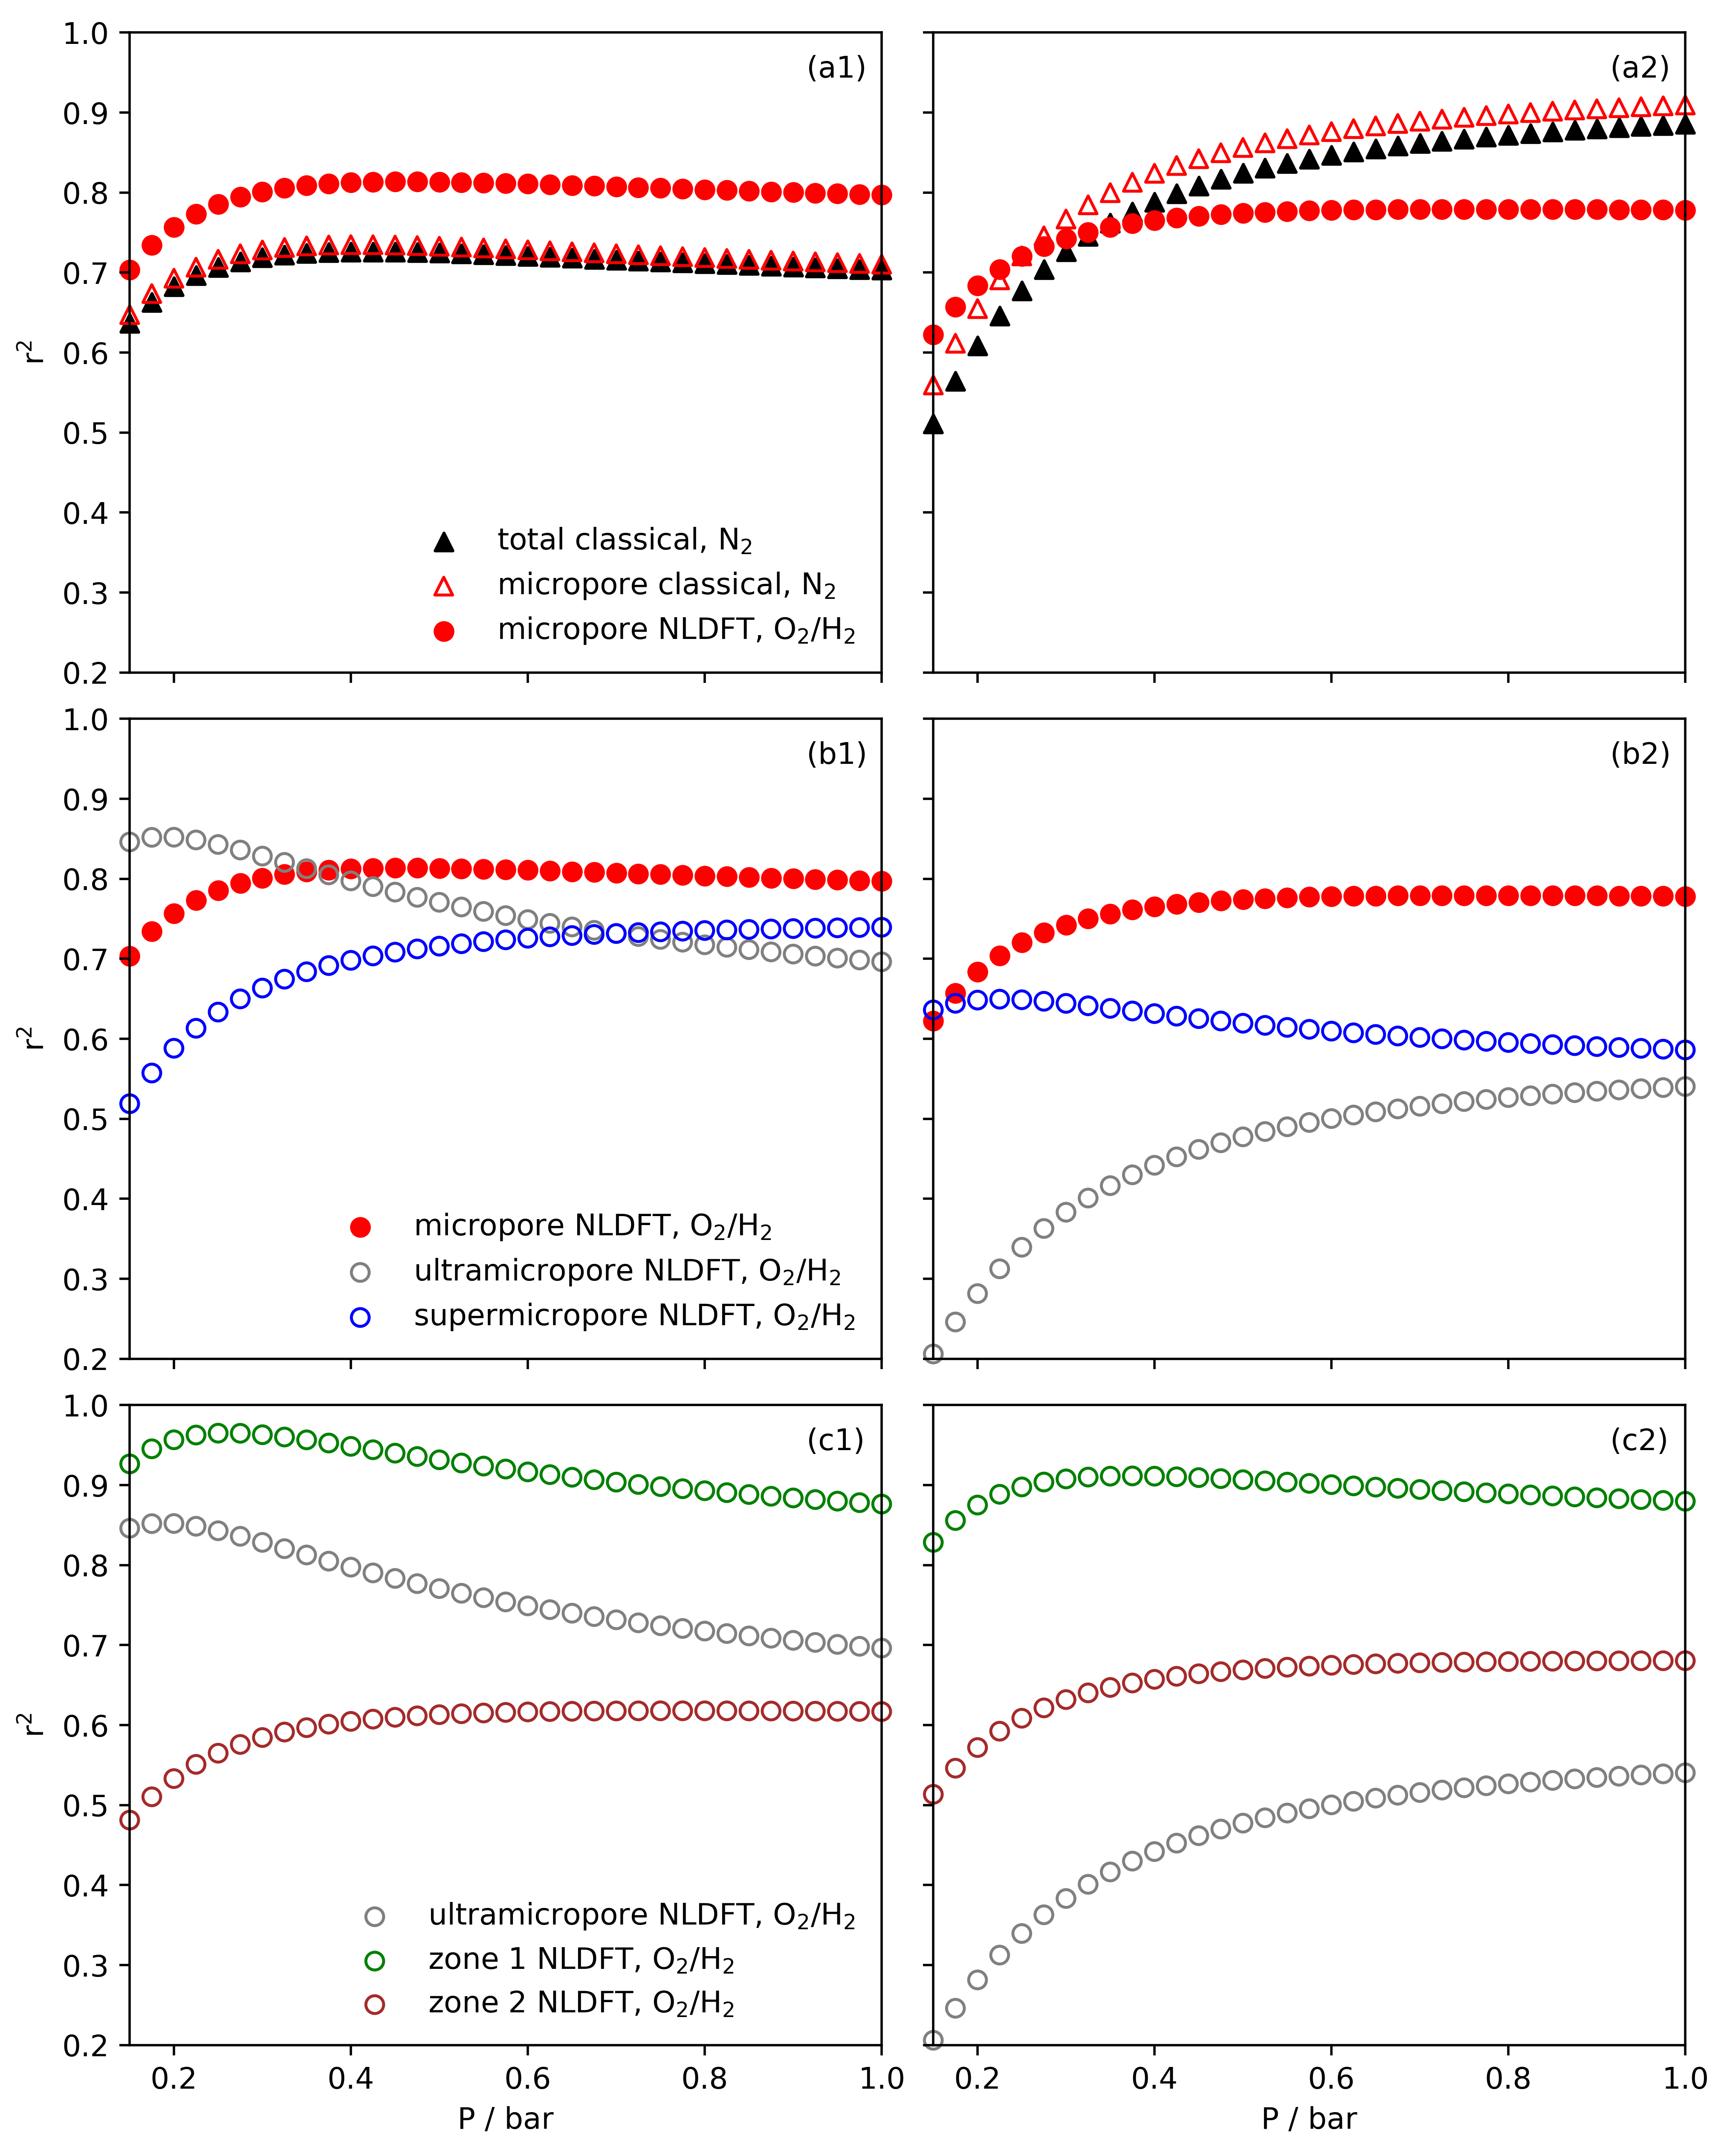
\includegraphics[width=\columnwidth, keepaspectratio]{6-pyPUC/figs/pyPUC_initial.png}
    \caption{Comparison of $r^2$ values derived from the linear regression of porosity as determined by different techniques and within differing pore width ranges against the gravimetric uptake (loading) of \ce{CO2} as a function of pressure. Linear regressions performed with using cumulative \acrshortpl{psd} and \ce{CO2} uptake isotherms of samples from section \ref{s:dual_initial}. Column (1) shows porosity in terms of surface area, and (2) in terms of pore volume. The classical microporosity values in (a1) and (a2) are derived using t-plot, whereas the total porosity is derived using the BET and  single point methods for surface area and pore volume respectively.}
    \label{fig:pyPUC_initial}
\end{figure}

The inconsistent results in terms of surface area and pore volume mentioned above may simply indicate the relative magnitude of the effects which surface area and pore volume of a material have on \gls{adsorption} capacity. Indeed, previous reports have only considered the relationship of pore volume below some pore width with \ce{CO2} uptake.\citep{Presser2011Effect, Sevilla2013Assessment, Adeniran2016Is, Wickramaratne2013Importance} This may be because surface area appears to have a relatively small influence on low pressure \ce{CO2} uptake\citep{Sevilla2021More, Ludwinowicz2015Effect, Singh2019CO2, GrauMarin2020Evaluation} - see \ref{pub:review}, \textbf{figure 3(a, c)}. However, when the \glspl{psd} are subdivided using the variable local minimum technique (see section \ref{s:dual_initial}), the results for both surface area and pore volume are far more consistent as shown in figure \ref{fig:pyPUC_initial}(c1, c2). In other words, both surface area and pore volume in region 1 - that is the pores of widths smaller than the local minimum - are strongly associated with \ce{CO2} uptake at all pressures below \qty{1}{\bar}. In fact $r^2$ values are highest at all pressures using this variable local minimum technique than for any of the other techniques shown in this figure. This indicates that these bimodal \acrshortpl{psd} may have some physical significance to the low-pressure uptake of \ce{CO2}.

In summary, these results indicate that the use of different sorptives can give radically different relationships between \gls{psd} and \ce{CO2} uptake as a function of pressure. This shows further applications of the pyPUC project, as the validity and utility of different porosimetric probes can be thoroughly investigated in their utility for determining optimum pore size range for \ce{CO2} uptake. While initial results are not conclusive, it appears that dual isotherm porosimetry may be important for understanding the relationship between pore size and \ce{CO2} uptake. While the variable local minimum method is impractical, subdividing the \gls{micropore} region at \qty{6.0}{\angstrom} may be more applicable to low pressure \ce{CO2} uptake. This is further investigated in \ref{pub:pyPUC}, \textbf{section 3.2}.

\section{Software Design}
\label{s:pypuc_design}
pyPUC is a fairly simple package whose structure is shown in figure \ref{fig:pyPUC_structure}. It is written almost exclusively in python,\citep{python1995} apart from one small bash script.\citep{bash2007} The main functions of pyPUC can be found in \verb|pyPUC/pyPUC/core|, while outside of this is the module \verb|pyPUC/interface.py| which constructs a simple command line interface to run the program, and the bash script \verb|pyPUC-cli| which executes \verb|pyPUC/interface.py|. Finally there is a directory for the \verb|source_data| which should be populated by the user with \acrshortpl{psd} and experimental uptake isotherms for the project in question.

\begin{figure}[ht!]
    \centering
    \begin{forest}
          for tree={
            font=\ttfamily,
            grow'=0,
            child anchor=west,
            parent anchor=south,
            anchor=west,
            calign=first,
            inner xsep=7pt,
            edge path={
              \noexpand\path [draw, \forestoption{edge}]
              (!u.south west) +(7.5pt,0) |- (.child anchor) pic {folder} \forestoption{edge label};
            },
            % style for your file node 
            file/.style={edge path={\noexpand\path [draw, \forestoption{edge}]
              (!u.south west) +(7.5pt,0) |- (.child anchor) \forestoption{edge label};},
              inner xsep=2pt,font=\small\ttfamily
                         },
            before typesetting nodes={
              if n=1
                {insert before={[,phantom]}}
                {}
            },
            fit=band,
            before computing xy={l=15pt},
          }  
        [pyPUC
          [pyPUC
            [core
              [best\_width\_at\_pressure.py,file]
              [psd\_processing.py,file]
              [uptake\_processing.py,file]
              [utils.py,file]
            ]
            [interface.py,file]
          ]
          [source\_data
            [project
              [psd
                [sorptive(s)]
              ]
              [uptake
                [sorptive]
              ]
            ]
          ]
          [pyPUC-cli,file]
        ]
    \end{forest}
    \caption{Structure of key modules and directories in the pyPUC package. There are other components in the github repository but they are not essential to the function of the package.}
    \label{fig:pyPUC_structure}
\end{figure}

The code is well documented, however a brief discussion of the purpose of each of the modules in \verb|pyPUC/pyPUC/core| follows here. Firstly \verb|utils.py| defines utility methods for the other three modules. Most important are the methods \verb|read_data()| and \verb|define_array()|. The former simply reads the data from the \verb|source_data| directory according to input arguments using the \verb|pandas| library,\citep{pandas2010} while the latter is a simple method for defining an array of pressures or pore widths for the modules \verb|uptake_processing| or \verb|psd_processing| using the \verb|numpy| library.\citep{numpy2022} 

\begin{table}[t!]
\centering
\captionof{table}{An example output of processed data from the \texttt{uptake\_processing.py} (a) and \texttt{psd\_processing.py} modules (b). \textit{A}, \textit{B}, \textit{C}, and \textit{D} are the four samples used in this analysis. In the case of (a), the numbers are the loadings of \ce{CO2} on the samples at each of the pressures in column \textit{p}, and for (b) they are the surface areas of the samples within the pore size range defined by $w_{min}$ and $w_{max}$.}
    \begin{subtable}{.5\linewidth}
      \centering
        \caption{}
        \begin{tabular}{l|l|l|l|l}
            p & A & B & C & D \\
            \midrule
            1 & 4.27 & 4.01 & 4.27 & 4.35 \\
            2 & 5.93 & 5.25 & 5.93 & 5.95 \\
            3 & 6.94 & 5.96 & 6.94 & 6.91 \\
        \end{tabular}
    \label{tb:loading_output}
    \end{subtable}%
    \begin{subtable}{.5\linewidth}
      \centering
        \caption{}
        \begin{tabular}{l|l|l|l|l|l}
            $\rm w_{min}$ & $\rm w_{max}$ & A & B & C & D \\
            \midrule
            5 & 4 & 59 & 282 & 238 & 260 \\
            6 & 4 & 401 & 514 & 442 & 465 \\
            6 & 5 & 142 & 232 & 204	& 204 \\
        \end{tabular}
    \label{tb:param_output}
    \end{subtable} 
\label{tb:loading_param_outputs}

\begin{python}
import pandas as pd
import numpy as np

sample_df = pd.read_csv('psd.csv')  # PSD stored in DataFrame 
w_array = [4, 5, 6]  # array of pore widths  
i=0
for wmax in w_array[1:]:  
    for wmin in w_array[w_array<wmax]:  # every possible combination of two w values
        rows_max = np.max(list(np.where(w < wmax)))
        rows_min = np.min(list(np.where(w > wmin)))
        max_value = sample_df.loc[rows_max, 'Vcum']
        min_value = sample_df.loc[rows_min, 'Vcum']
        param = max_value - min_value
        i+=1 # Go through all possible values of wmin for wmax
\end{python}
\captionof{figure}{How the porosity within some pore width range is determined in pyPUC. Note that this is pseudo-code\citep{davis2019pseudocode} as opposed to the actual source code.}
\label{fig:pypuc_porosity}
\end{table}

The \verb|uptake_processing.py| and \verb|psd_processing.py| modules are fairly self-explanatory, in each case simply processing the uptake or \acrshort{psd} data for all samples in \verb|source_data/project|. The outputs from these modules can be seen in figure \ref{tb:loading_param_outputs}. The former attempts to fit each uptake isotherm in the appropriate project in \verb|source_data| to a range of model isotherms and selects the best fit, by using the \verb|modelling| module from the library \verb|pygaps|.\citep{Iacomi2019pyGAPS} These model isotherms are then converted to point isotherms at pressures defined by the user. The pressures and loadings are then stored in a two-dimensional DataFrame, $D_\upsilon$ (see table \ref{tb:loading_output}). The latter reads in the cumulative \acrshortpl{psd} for each sample, and determines the pore volume or surface area within each user-defined pore size range. A demonstration of how this works is shown in figure \ref{fig:pypuc_porosity}. This is done for each sample and stored in the DataFrame $D_\pi$ (see table \ref{tb:param_output}). In either case, the data produced can be stored in memory or output as a \verb|.csv|, alongside a simple report of the data processing as shown in the appendix, figures \ref{fig:loading_report} and \ref{fig:psd_report}.

Finally \verb|best_width_at_pressure.py| takes the two DataFrames generated by \verb|uptake_processing.py| and \verb|psd_processing.py| and uses the \verb|stats.linregress()| method from the \verb|scipy| library\citep{SciPy2020} to perform linear regressions between each row of $D_\upsilon$ and each row of $D_\pi$. That is, if each of $D_\upsilon$ and $D_\pi$ have three rows (1, 2, 3) then a linear regression of row 1 in $D_\upsilon$ will be performed against each row 1, 2 and 3 of $D_\pi$. Then the same is performed for row 2 of $D_\upsilon$, etc.. \verb|scipy.stat.linregress()| then returns the $r^2$ value, slope, and intercept of the regression which is stored in the correlation DataFrame, $D_c$ alongside the values for $w_{min}$, $w_{max}$ and $P$ - an example of this can be seen in table \ref{tb:D_c}. $D_c$ can be reduced in size using the method \verb|correlation_requirements()| which allows rows in the DataFrame to be eliminated according to various arguments. The best pair of $w_{min}$ and $w_{max}$, according to the highest $r^2$ value for each pressure can be selected using the method \verb|make_correlation_df()|, i.e. yielding the optimum pore size region for uptake of the sorptive, $\Omega$.

\begin{table}[h!]
    \centering
    \begin{tabular}{l|l|l|l|l|l|l|l}
        $\rm w_{min}$ & $\rm w_{max}$ & p & $\rm r^2$ & m & c & x & y \\
        \midrule
        \rowcolor{yellow} 4 & 5 & 1 & 0.503 & -0.005 & 5.77 & [259 282 ...] & [4.27 4.01 ...] \\
        \rowcolor{yellow} 4 & 5 & 2 & 0.667 & -0.0157	& 9.85 & [259 282 ...] & [5.93 5.25 ...] \\
        4 & 5 & 3 & 0.691 & -0.0225 & 12.5 & [259 282 ...] & [6.94 5.96 ...] \\
        4 & 6 & 1 & 0.457 & -0.00213 & 5.20 & [401 514 ...] & [4.27 4.01 ...] \\
        4 &	6 & 2 & 0.662 & -0.00591 & 8.46	& [401 514 ...] & [5.93 5.25 ...] \\
        \rowcolor{yellow} 4 &	6 & 3 &	0.696 & -0.00854 & 10.5 & [401 514 ...] & [6.94 5.96 ...] \\
        5 & 6 & 1 & 0.254 & -0.00196 & 4.61 & [142 232 ...] & [4.27 4.01 ...] \\
        5 & 6 & 2 & 0.390 & -0.00561 & 6.86 & [142 232 ...] & [5.93 5.25 ...] \\
        5 & 6 & 3 & 0.413 & -0.00814 & 8.28 & [142 232 ...] & [6.94 5.96 ...] \\
    \end{tabular}
    \caption{Example output of a $D_c$ DataFrame from \ce{CO2} uptake and \acrshort{psd} data in table \ref{tb:loading_param_outputs}. Highlighted rows indicate the regression that yields the optimum pore size range ($\Omega$) for each of the pressures (1, 2, and 3 bar). Columns x and y indicate the surface area and loadings used for the regression, respectively. Values are truncated to save space.}
    \label{tb:D_c}
\end{table}

\newpage
\section[Publication III]{\texorpdfstring{Publication III: Brute force determination of the optimum pore sizes for
\ce{CO2} uptake}{Publication III: Brute force determination of the optimum pore sizes for
CO2 uptake}}

\textbf{Contribution of the author}: The author came up with the concept of the pyPUC software, designed and implemented it, and performed all analyses. A portion of the experimental work necessary to create DataSet 1, and all experimental work for DataSet 2 was also done by the author. The author wrote the paper in its entirety.

\setcounter{opagenum}{\thepage}

\newpage

\setlength{\originalVOffset}{\voffset}   
\setlength{\originalHOffset}{\hoffset}

\setlength{\voffset}{0cm}
\setlength{\hoffset}{0cm}
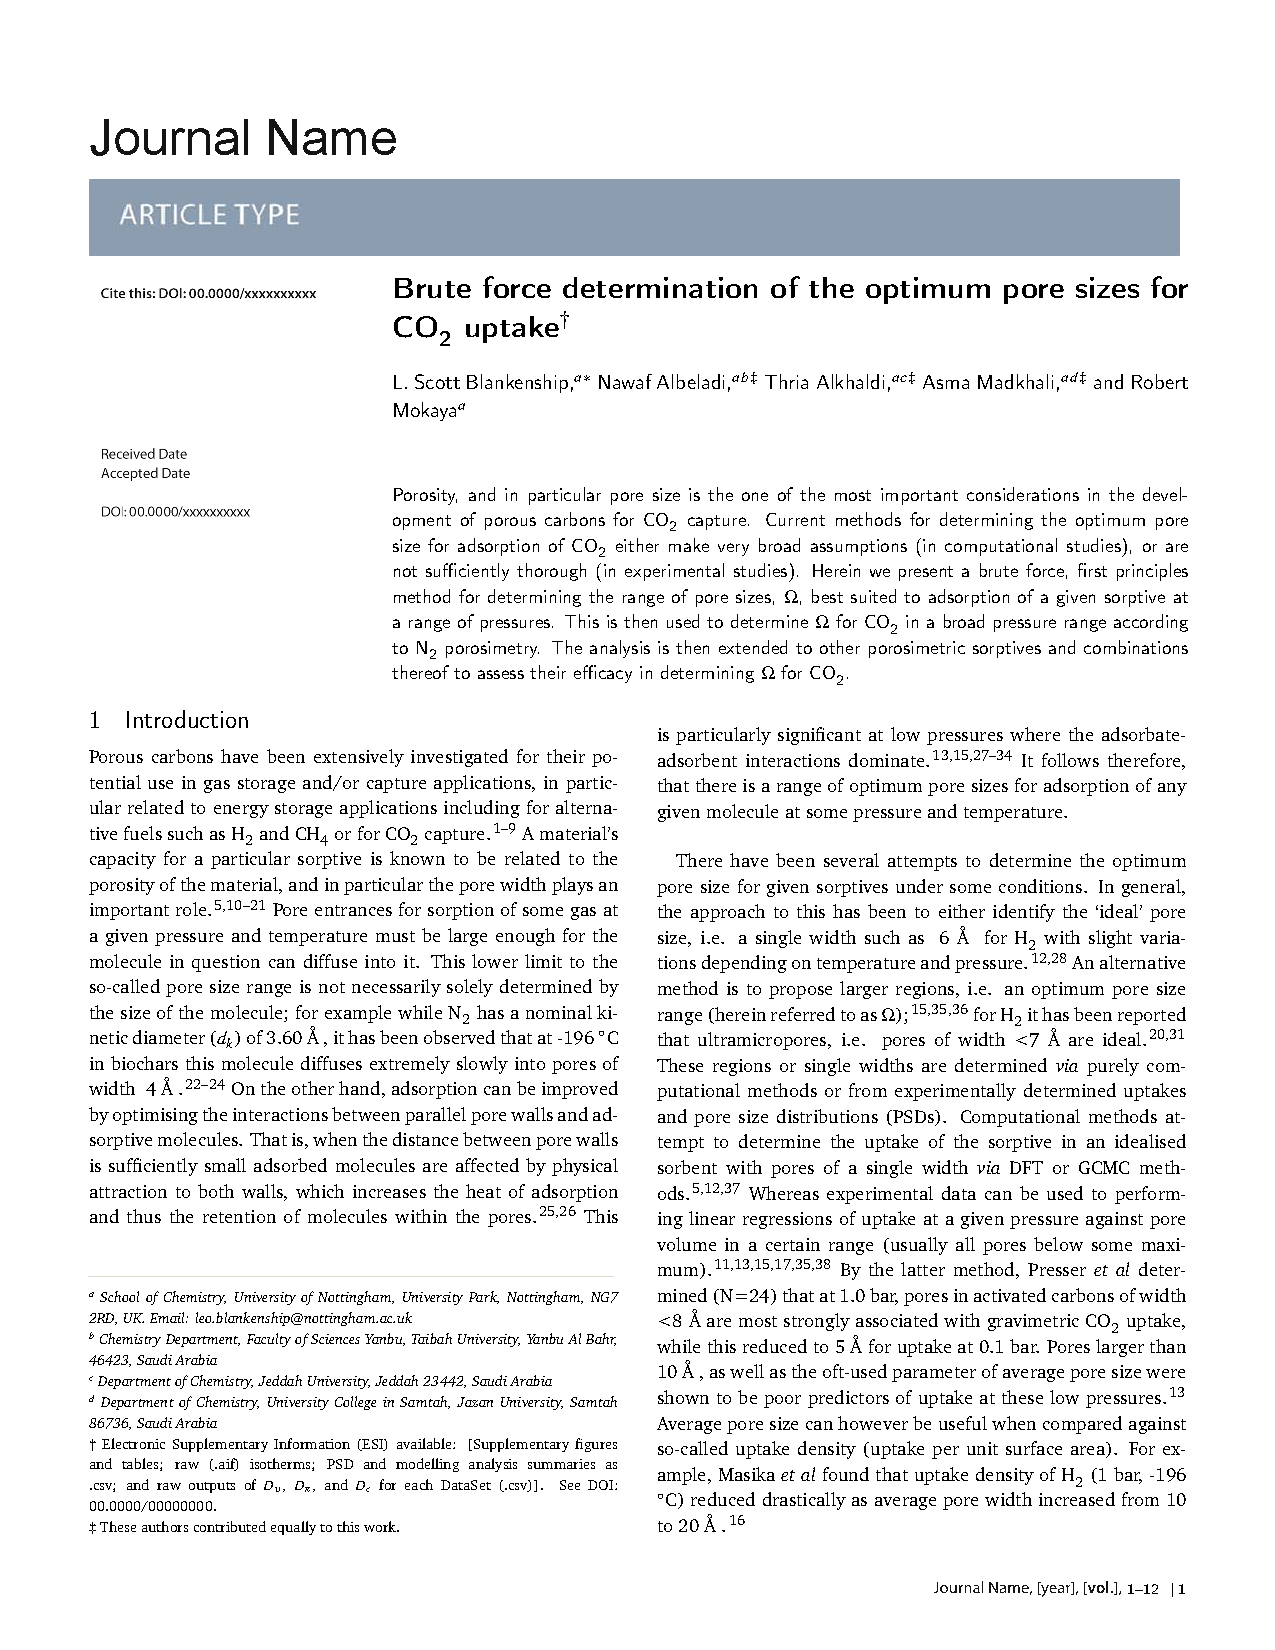
\includepdf[pagecommand={
    \setcounter{page}{\theopagenum}
    \thispagestyle{empty}
    },
    pages=-]{6-pyPUC/publication_03.pdf}
\setlength{\voffset}{\originalVOffset}
\setlength{\hoffset}{\originalHOffset}

%%%%Placeholder
%\section{\texorpdfstring{Describing porosity and pressure dependent \ce{CO2} uptake relationships mathematically}{Describing porosity and pressure dependent CO2 uptake relationships mathematically}}

%\begin{equation}
%    r^2 \left(P,\,w_{max} \right) = \dfrac{A}{P}\exp{\dfrac{\ln{\frac{P}{\mu_g}}}{2\left(\ln{\sigma_g}\right)^2}}
%\end{equation}

%\begin{equation}
%    \sigma_g \left(w_{max}\right) = \sigma_{g(0)}\exp{\left( -\lambda\, w_{max} \right)} + c 
%\end{equation}
%%%%Placeholder

\section{Summary \& Future Work}
The \acrshort{pypuc} method is a thorough, intuitive, and assumption-less route to understanding the relationship between \gls{adsorbent} pore size and physisorptive uptake capacity of some \gls{adsorbate}. It expands upon both purely computational and purely experimental methods by performing a broad analysis of the correlation (\textit{via} the Pearson coefficient, $r^2$) of porosity within pores of some range of widths and \gls{adsorbate} uptake at some pressure. Its utility has been demonstrated in \ref{pub:pyPUC} with \ce{CO2} on \glspl{turbostratic carbon}, with porosity derived from \ce{N2} isotherms as well as by comparing results derived using \acrshortpl{psd} from different porosimetric \glspl{adsorbate}.

The relationship between \ce{CH4} uptake in \glspl{turbostratic carbon} and pore size is one of the least well understood in the field of small gas molecule capture and storage.\citep{Matranga1992Molecular, Tan1990Adsorption, Simon2015materials, Biloe2002Optimal} This problem should be considered a priority for the use of pyPUC - indeed as \ce{CH4} is a non-polar molecule and larger than \ce{CO2},\citep{Breck1974Zeolite, Poling2001Properties} results from this analysis should be less influenced by carbon surface chemistry and very small \glspl{ultramicropore} and thus may provide a simpler understanding of the relationship between pore size and pressure-dependent gas uptake. Similarly pyPUC ought to be applied to \ce{H2} storage; while the relationship between pore size and \ce{H2} uptake capacity is perhaps one of the best understood, the analysis could provide some interesting insights. However, this could be problematic in that the general consensus is that optimum pore size for \ce{H2} uptake is \qty{6.0}{\angstrom}\citep{DelaCasaLillo2002Hydrogen, Cabria2007optimum} so porosity ought to be probed by a small sorptive like \ce{H2} - it could be considered unreasonable to determine porosity with the same molecule for which the materials' uptake capacity is being assessed.

pyPUC currently only considers the uptake capacity in the derivation of the $\Omega$. In the future, pyPUC should be expanded to include isosteric heat of \gls{adsorption} $q_{st}$ as a variable. While $q_{st}$ is typically determined using the Clausius-Clapeyron method,\citep{clausius1850ueber, clapeyron1834memoire} the analysis could perhaps be made more efficient by employing the Whittaker method which has been shown to yield comparable results and only requires a single isotherm.\citep{whittaker2013predicting, li2018adsorption} pyPUC could then be used to derive a relationship between porosity in some range of pore sizes and $q_{st}$.

\newpage
\section[Publication III Supporting Information]{\texorpdfstring{Publication III Supporting Information: Brute force determination of the optimum pore sizes for \ce{CO2} uptake}{Publication III Supporting Information: Brute force determination of the optimum pore sizes for CO2 uptake}}

\setcounter{opagenum}{\thepage}

\newpage

\setlength{\originalVOffset}{\voffset}   
\setlength{\originalHOffset}{\hoffset}

\setlength{\voffset}{0cm}
\setlength{\hoffset}{0cm}
\includepdf[pagecommand={
    \setcounter{page}{\theopagenum}
    \thispagestyle{empty}
    },
    pages=-]{6-pyPUC/si_03.pdf}
\setlength{\voffset}{\originalVOffset}
\setlength{\hoffset}{\originalHOffset}

\bibliographystyle{rsc}
\bibliography{bibliography/bib.bib}